%% ------------------------------------------------------------------------- %%
\chapter{Ajuste dos hiper-parâmetros e normalização em lote}
\label{ape:ajuste-hiper-parametros-cnn}

Neste capítulo apresentamos os resultados dos ajustes dos hiper-parâmetros e da normalização em lote feita nas arquiteturas convolucional, \Gls{unif} e \textit{Embedding}. O intuito destes ajustes é obter um modelo mais robusto e evitar o \textit{overfitting}.

\section{Ajuste dos hiper-parâmetros da rede convolucional}
\label{sec:ajuste-hiper-parametros-cnn}

A rede convolucional exige alguns hiper-parâmetros que devem ser informados durante o treinamento. O tamanho da entrada, conforme citado no capítulo~\ref{cap:experimento}, foi fixado em 150. Caso as palavras tenham tamanho menor, o vetor é preenchido com valores $0$ ao final. Outros três parâmetros exigidos pela rede convolucional são: filtros, kernel e stride.

O parâmetro kernel define o tamanho da janela de operação de convolução. No nosso caso, que estamos utilizando a operação de convolução de 1 dimensão, Conv1D, o kernel define os n-grams a ser extraídos do vetor de entrada. 
O parâmetro filtros define a dimensão de saída da operação de convolução. Este parâmetro indica a quantidade de filtros no resultado da operação de convolução. Cada filtro tenta extrair uma característica diferente do vetor de entrada. E o parâmetro stride define a quantidade de posições de deslocamento do filtro. O parâmetro stride foi fixado em 1. Neste caso, o filtro desloca-se por todas as posições do vetor de entrada de uma em uma posição.

Fizemos alguns testes com relação a quantidade de filtros e o tamanho do kernel utilizando como base os experimentos feitos por \cite{feng-2015} e \cite{tan-lstm-qa}. Tanto \cite{feng-2015} quanto \cite{tan-lstm-qa} utilizaram o parâmetro filtros com o valor entre 1000 e 4000. Em nossos testes, além destes valores, analisamos também os filtros para valores menores como 50, 100, 200 e 500. Já o tamanho do kernel, \cite{tan-lstm-qa} utilizou o valor 2. Em nossos testes, variamos o valor entre 2 e 4, além de concatenar kernels de diferentes valores, combinando kernels de tamanhos 2, 3, 5 e 7.

\subsection{Filtros}

Inicialmente, analisamos o comportamento da rede convolucional proposta no caítulo~\ref{cap:experimento} (ver Figura~\ref{fig:cnn-architecture}) utilizando diferentes quantidades de filtros. Nas figuras a seguir, exibimos um gráfico de comparação do valor do erro no conjunto de treinamento em comparação com o erro no conjunto de validação. Conforme citado no capítulo~\ref{cap:experimento}, foram utilizadas $60.083$ amostras, sendo que $42058$ foram utilizadas para o conjunto de treinamento e $18025$ para o conjunto de validação. Neste experimento, analisamos as seguintes quantidades de filtros: 50, 100, 200, 500, 1000, 2000, 4000. Inicialmente, utilizamos o kernel com o valor 2, valor recomendado por \cite{tan-lstm-qa}.

\begin{figure}[p]
\begin{subfigure}{.5\textwidth}
  \centering
  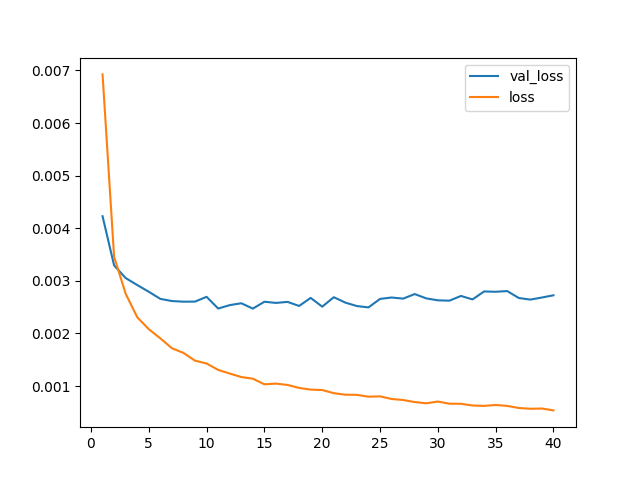
\includegraphics[width=.8\linewidth]{figuras/ape-ajustes-hiper-parametros/cnn-50-k-2.png}
  \caption{Rede convolucional com parâmetro $F = 50$}
  \label{fig:cnn-50-k-2}
\end{subfigure}%
\begin{subfigure}{.5\textwidth}
  \centering
  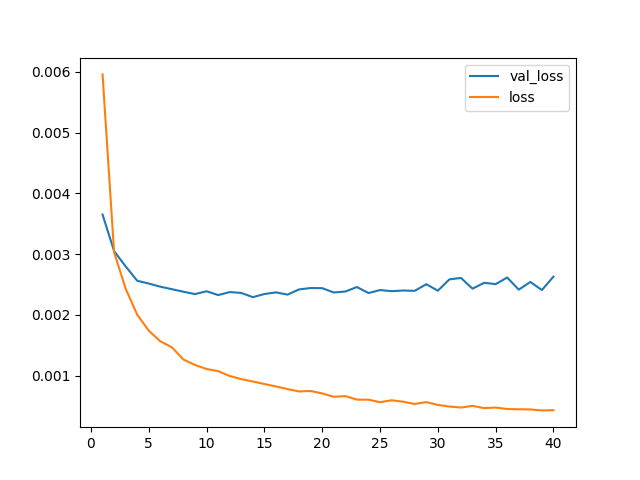
\includegraphics[width=.8\linewidth]{figuras/ape-ajustes-hiper-parametros/cnn-100-k-2.png}
  \caption{Rede convolucional com parâmetro $F = 100$}
  \label{fig:cnn-100-k-2}
\end{subfigure}
\begin{subfigure}{.5\textwidth}
  \centering
  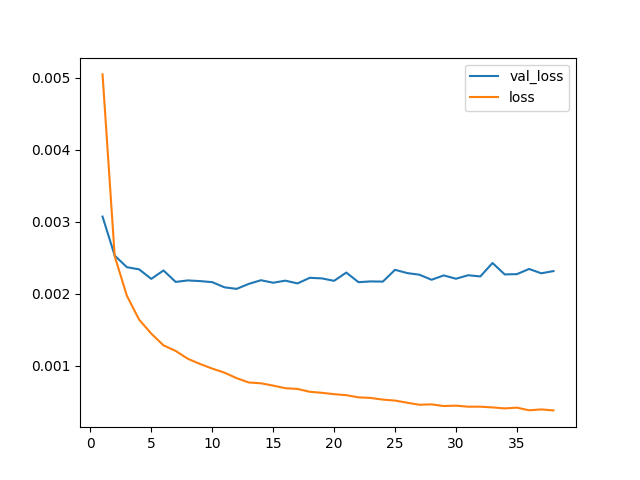
\includegraphics[width=.8\linewidth]{figuras/ape-ajustes-hiper-parametros/cnn-200-k-2.png}
  \caption{Rede convolucional com parâmetro $F = 200$}
  \label{fig:cnn-200-k-2}
\end{subfigure}
\begin{subfigure}{.5\textwidth}
  \centering
  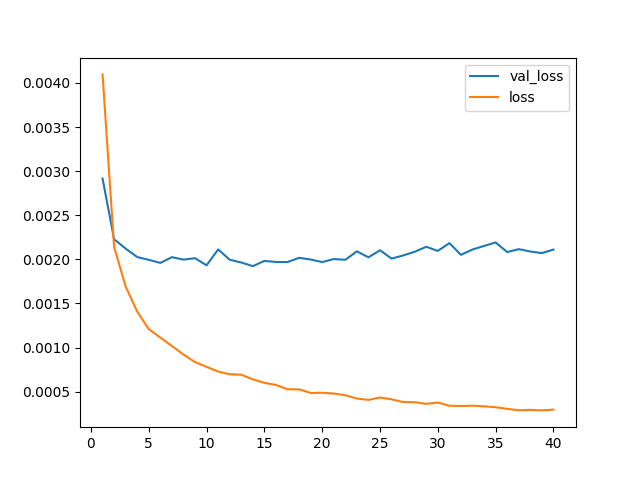
\includegraphics[width=.8\linewidth]{figuras/ape-ajustes-hiper-parametros/cnn-500-k-2.png}
  \caption{Rede convolucional com parâmetro $F = 500$}
  \label{fig:cnn-500-k-2}
\end{subfigure}
\begin{subfigure}{.5\textwidth}
  \centering
  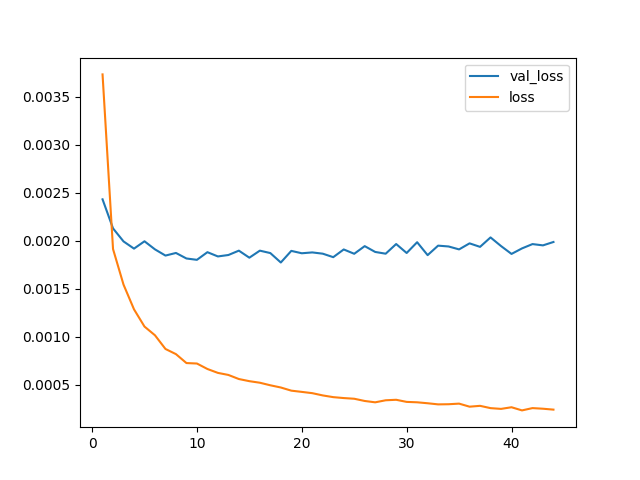
\includegraphics[width=.8\linewidth]{figuras/ape-ajustes-hiper-parametros/cnn-1000-k-2.png}
  \caption{Rede convolucional com parâmetro $F = 1000$}
  \label{fig:cnn-1000-k-2}
\end{subfigure}
\begin{subfigure}{.5\textwidth}
  \centering
  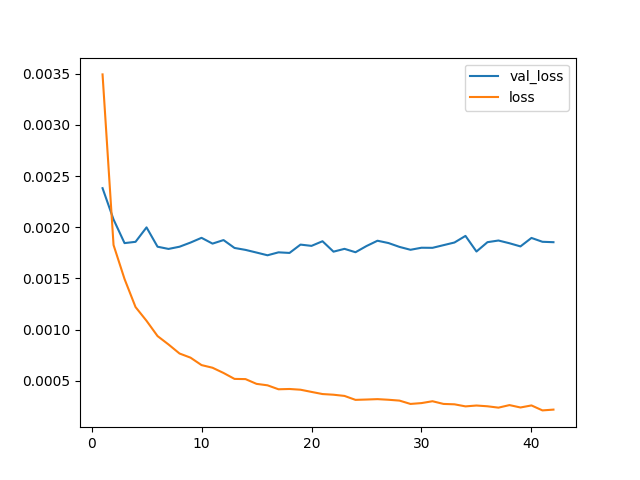
\includegraphics[width=.8\linewidth]{figuras/ape-ajustes-hiper-parametros/cnn-2000-k-2.png}
  \caption{Rede convolucional com parâmetro $F = 2000$}
  \label{fig:cnn-2000-k-2}
\end{subfigure}
\begin{subfigure}{.5\textwidth}
  \centering
  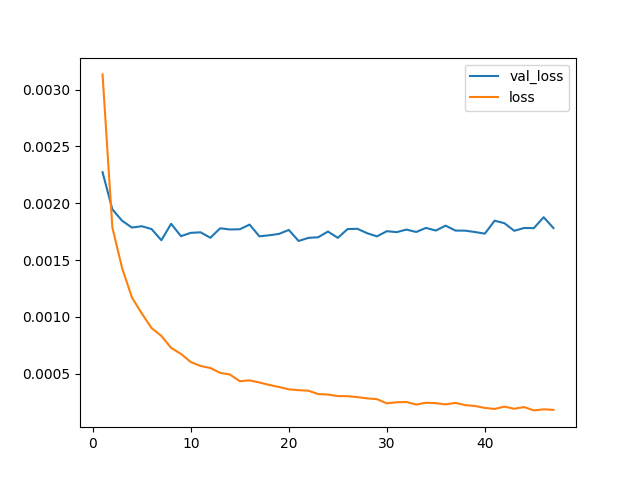
\includegraphics[width=.8\linewidth]{figuras/ape-ajustes-hiper-parametros/cnn-4000-k-2.png}
  \caption{Rede convolucional com parâmetro $F = 4000$}
  \label{fig:cnn-4000-k-2}
\end{subfigure}
\caption{Este gráfico apresenta um comparativo do erro no conjunto de validação em comparação com o erro no conjunto de treinamento. Mais detalhes sobre o treinamento, ver a Seção~\ref{sec:treinamento}. Arquitetura de rede convolucional proposta no Capítulo~\ref{cap:abordagem}, ver Figura~\ref{fig:cnn-architecture}. Hiper-parâmetros: $m = 0.009$, $k = 2$. O parâmetro F indica a quantidade de filtros convolucionais. Nas figuras de \emph{a} a \emph{g}, o eixo \emph{y} indica o valor de erro da função de perda \textit{hinge}, já o eixo \emph{x} indica as épocas de treinamento. A legenda \emph{val\_loss} das figuras de \emph{a} a \emph{g} indica o erro na amostra de validação e a legenda \emph{loss} indica o valor do erro na amostra de treinamento. }
\label{fig:treinamento-cnn-k-2-m-0009}
\end{figure}

De acordo com a Figura~\ref{fig:treinamento-cnn-k-2-m-0009}, o aumento de filtros diminuiu o valor do erro na amostra de validação. O valor de erro que era em torno de $0,003$ na Figura~\ref{fig:cnn-50-k-2}, diminui pela metade, ficando em torno de $0.0015$ nas Figuras~\ref{fig:cnn-2000-k-2} e \ref{fig:cnn-4000-k-2}. O aumento da quantidade de filtros aumenta a capacidade do modelo, pois quanto mais filtros, mais características latentes a rede convolucional tentará extrair dos dados. No nosso caso, isto refletiu no resultado na amostra de validação, diminuindo o valor do erro. Porém, podemos observar que o comportamento do modelo começa a dar sinais de \textit{overfitting}, onde o valor do erro na amostra de treinamento cai abruptamente, enquanto o erro na amostra de validação permance estável e começa a aumentar. Para lidar com este problema, utilizamos normalização em lote e apresentamos os resultados na Seção~\ref{sec:regularizacao-normalizacao-lote}. 

\subsection{Kernel}

Conforme exibido no Capítulo~\ref{cap:abordagem}, o kernel define na rede convolucional de 1 dimensão, o n-grams a serem extraídos. Durante o treinamento, analisamos diferentes valores para o kernel. Verificamos o comportamento para kernel de tamanho 2, 3, 4 e a combinação de valores 2, 3, 5 e 7. Conforme as Figuras~\ref{fig:treinamento-cnn-diferentes-kernels} e \ref{fig:treinamento-cnn-diferentes-kernels-2}, não houve melhora significativa para kernels de tamanho 3 e 4 em comparação com o kernel de tamanho 2. E até mesmo a combinação de kernels não gerou uma melhora significativa dado a quantidade de parâmetros utilizados. Neste caso, optamos por manter o kernel fixado em $2$.


\begin{figure}[p]
\begin{subfigure}{.5\textwidth}
  \centering
  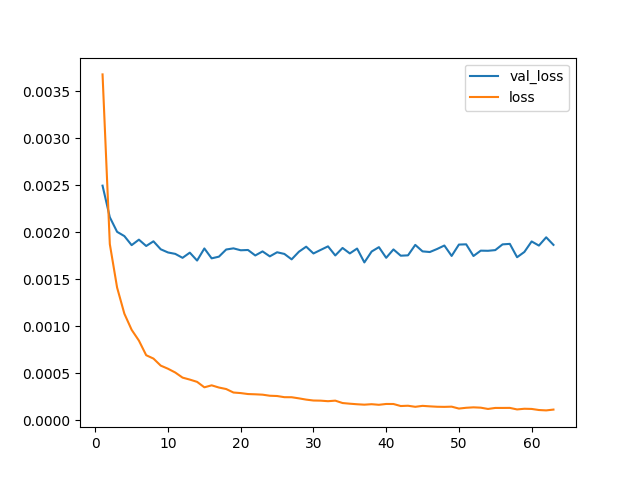
\includegraphics[width=.8\linewidth]{figuras/ape-ajustes-hiper-parametros/cnn-1000.png}
  \caption{Rede convolucional com parâmetro $F = 1000$ e $K = [2,3,5,7]$}
  \label{fig:cnn-1000}
\end{subfigure}%
\begin{subfigure}{.5\textwidth}
  \centering
  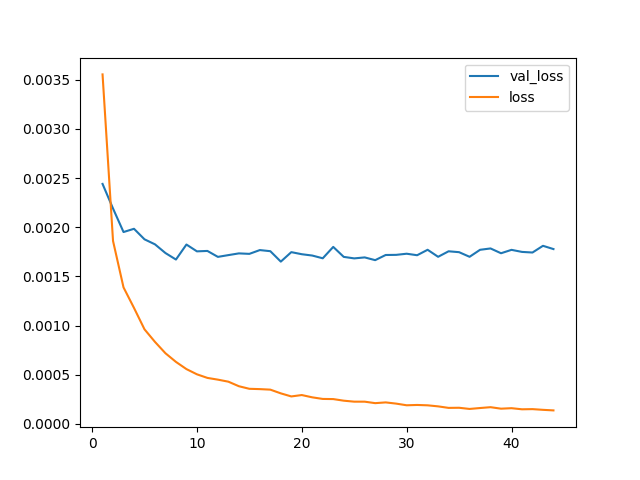
\includegraphics[width=.8\linewidth]{figuras/ape-ajustes-hiper-parametros/cnn-2000.png}
  \caption{Rede convolucional com parâmetro $F = 2000$ e $K = [2, 3, 5, 7]$}
  \label{fig:cnn-2000}
\end{subfigure}
\begin{subfigure}{.5\textwidth}
  \centering
  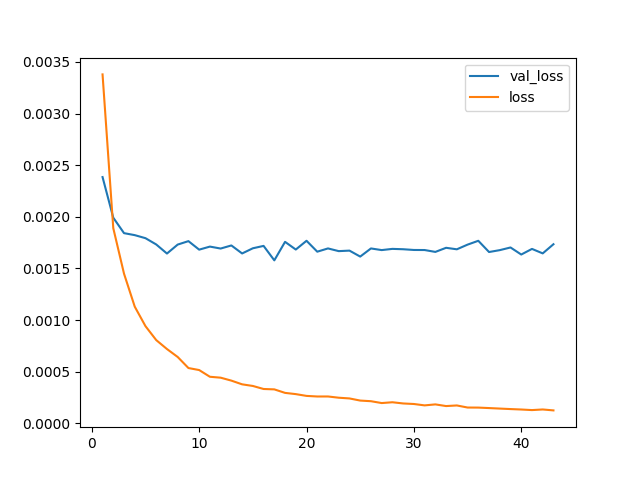
\includegraphics[width=.8\linewidth]{figuras/ape-ajustes-hiper-parametros/cnn-4000.png}
  \caption{Rede convolucional com parâmetro $F = 4000$ e $K = [2, 3, 5, 7]$}
  \label{fig:cnn-4000}
\end{subfigure}
\begin{subfigure}{.5\textwidth}
  \centering
  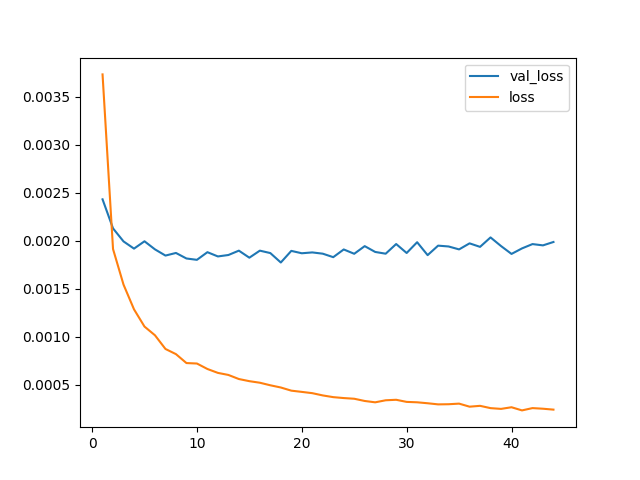
\includegraphics[width=.8\linewidth]{figuras/ape-ajustes-hiper-parametros/cnn-1000-k-2.png}
  \caption{Rede convolucional com parâmetro $F = 1000$ e $K = 2$}
  \label{fig:cnn-1000-k-2-v2}
\end{subfigure}
\begin{subfigure}{.5\textwidth}
  \centering
  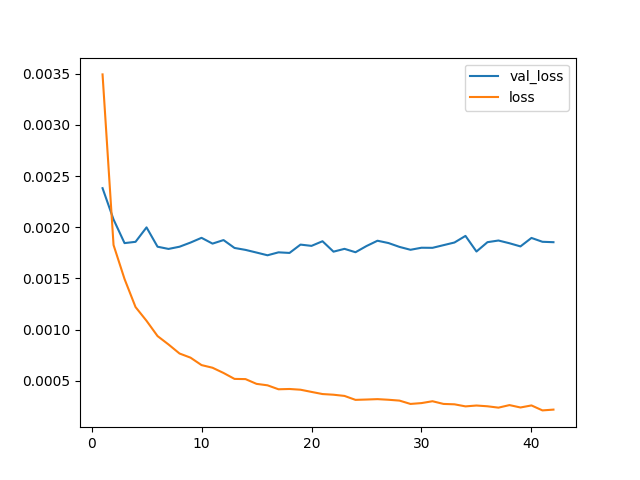
\includegraphics[width=.8\linewidth]{figuras/ape-ajustes-hiper-parametros/cnn-2000-k-2.png}
  \caption{Rede convolucional com parâmetro $F = 2000$ e $K = 2$}
  \label{fig:cnn-2000-k-2-v2}
\end{subfigure}
\begin{subfigure}{.5\textwidth}
  \centering
  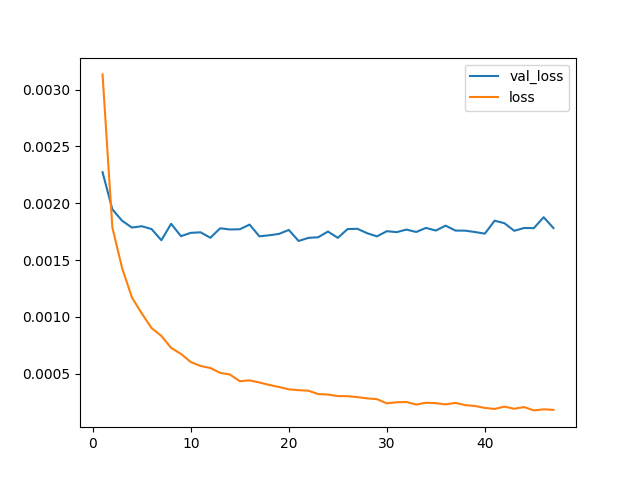
\includegraphics[width=.8\linewidth]{figuras/ape-ajustes-hiper-parametros/cnn-4000-k-2.png}
  \caption{Rede convolucional com parâmetro $F = 4000$ e $K = 2$}
  \label{fig:cnn-4000-k-2-v2}
\end{subfigure}
\caption{Gráfico do treinamento da rede convolucional na recuperação de trecho de código-fonte. Este gráfico apresenta um comparativo do erro no conjunto de validação em comparação com o erro no conjunto de treinamento. Mais detalhes sobre o treinamento, ver a Seção~\ref{sec:treinamento}. Arquitetura de rede convolucional proposta no Capítulo~\ref{cap:abordagem}, ver Figura~\ref{fig:cnn-architecture}. Hiper-parâmetros: $m = 0.009$. O parâmetro F indica a quantidade de filtros convolucionais, o parâmetro K indica o tamanho da janela do filtro convolucional. Nas figuras de \emph{a} a \emph{f}, o eixo \emph{y} indica o valor de erro da função de perda \textit{hinge}, já o eixo \emph{x} indica as épocas de treinamento. A legenda \emph{val\_loss} das figuras de \emph{a} a \emph{g} indica o erro na amostra de validação e a legenda \emph{loss} indica o valor do erro na amostra de treinamento. }
\label{fig:treinamento-cnn-diferentes-kernels}
\end{figure}

\begin{figure}[p]
\begin{subfigure}{.5\textwidth}
  \centering
  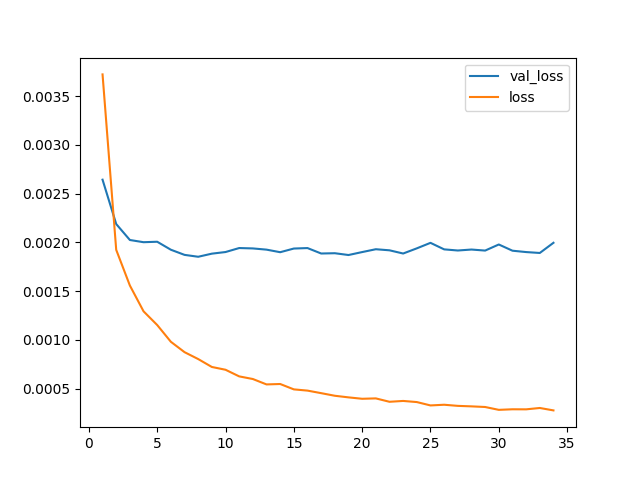
\includegraphics[width=.8\linewidth]{figuras/ape-ajustes-hiper-parametros/cnn-1000-k-3.png}
  \caption{Rede convolucional com parâmetro $F = 1000$ e $K = 3$}
  \label{fig:cnn-1000-k-3}
\end{subfigure}
\begin{subfigure}{.5\textwidth}
  \centering
  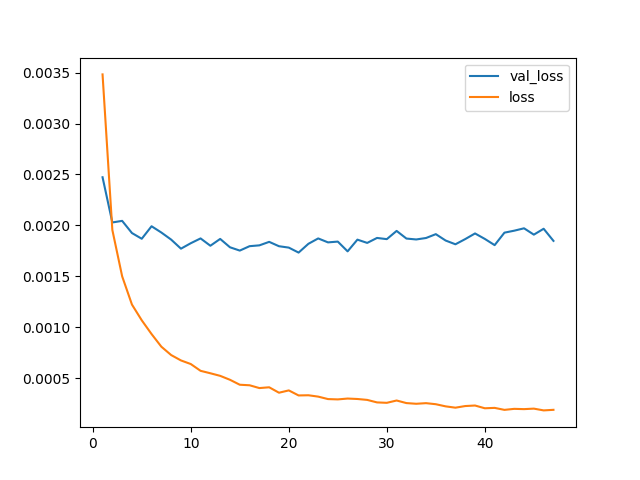
\includegraphics[width=.8\linewidth]{figuras/ape-ajustes-hiper-parametros/cnn-2000-k-3.png}
  \caption{Rede convolucional com parâmetro $F = 2000$ e $K = 3$}
  \label{fig:cnn-2000-k-3}
\end{subfigure}
\begin{subfigure}{.5\textwidth}
  \centering
  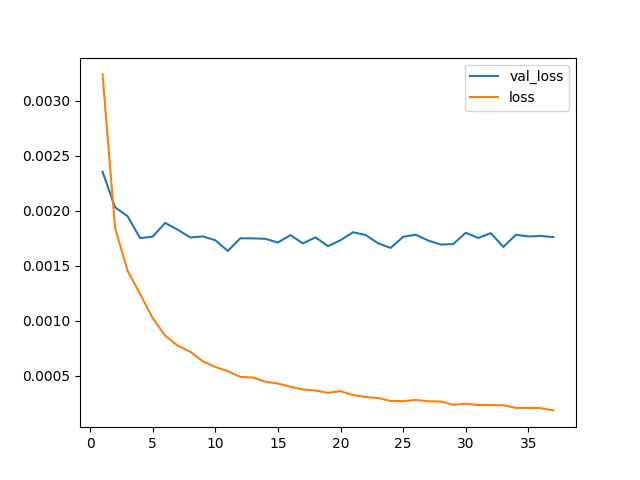
\includegraphics[width=.8\linewidth]{figuras/ape-ajustes-hiper-parametros/cnn-4000-k-3.png}
  \caption{Rede convolucional com parâmetro $F = 4000$ e $K = 3$}
  \label{fig:cnn-4000-k-3}
\end{subfigure}
\begin{subfigure}{.5\textwidth}
  \centering
  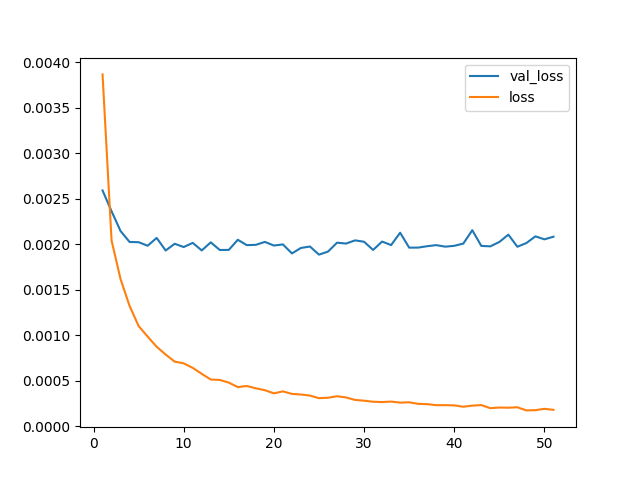
\includegraphics[width=.8\linewidth]{figuras/ape-ajustes-hiper-parametros/cnn-1000-k-4.png}
  \caption{Rede convolucional com parâmetro $F = 1000$ e $K = 4$}
  \label{fig:cnn-1000-k-4}
\end{subfigure}
\begin{subfigure}{.5\textwidth}
  \centering
  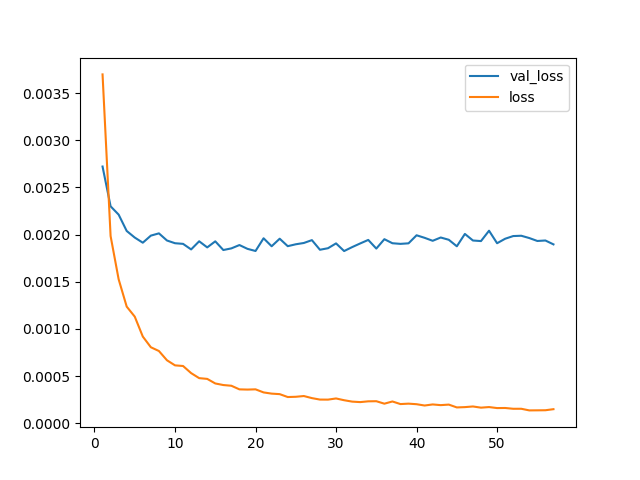
\includegraphics[width=.8\linewidth]{figuras/ape-ajustes-hiper-parametros/cnn-2000-k-4.png}
  \caption{Rede convolucional com parâmetro $F = 2000$ e $K = 4$}
  \label{fig:cnn-2000-k-4}
\end{subfigure}
\begin{subfigure}{.5\textwidth}
  \centering
  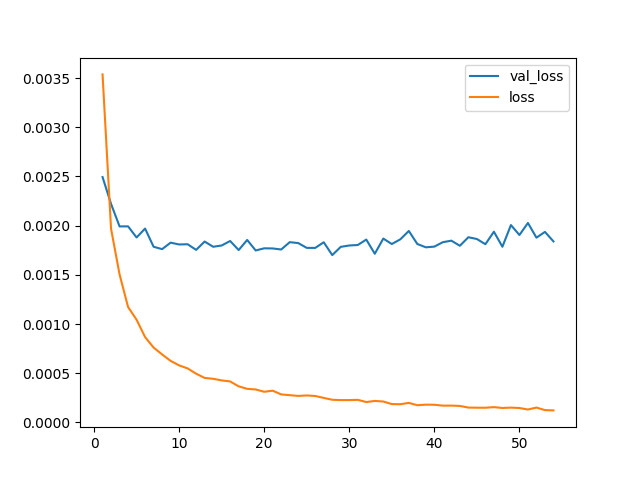
\includegraphics[width=.8\linewidth]{figuras/ape-ajustes-hiper-parametros/cnn-4000-k-4.png}
  \caption{Rede convolucional com parâmetro $F = 4000$ e $K = 4$}
  \label{fig:cnn-4000-k-4}
\end{subfigure}
\caption{Gráfico do treinamento da rede convolucional na recuperação de trecho de código-fonte. Este gráfico apresenta um comparativo do erro no conjunto de validação em comparação com o erro no conjunto de treinamento. Mais detalhes sobre o treinamento, ver a Seção~\ref{sec:treinamento}. Arquitetura de rede convolucional proposta no Capítulo~\ref{cap:abordagem}, ver Figura~\ref{fig:cnn-architecture}. Hiper-parâmetros: $m = 0.009$. O parâmetro F indica a quantidade de filtros convolucionais, o parâmetro K indica o tamanho da janela do filtro convolucional. Nas figuras de \emph{a} a \emph{f}, o eixo \emph{y} indica o valor de erro da função de perda \textit{hinge}, já o eixo \emph{x} indica as épocas de treinamento. A legenda \emph{val\_loss} das figuras de \emph{a} a \emph{g} indica o erro na amostra de validação e a legenda \emph{loss} indica o valor do erro na amostra de treinamento. }
\label{fig:treinamento-cnn-diferentes-kernels-2}
\end{figure}



\section{Ajuste da margem - Função de perda hinge}

\section{Regularização - Normalização em Lote}
\label{sec:regularizacao-normalizacao-lote}



